\documentclass[10pt, titlepage]{article}

\usepackage{graphicx}
\graphicspath{ {../build/img/} }

\begin{document}

\title{Cardie Static UI Report}

\author{Daanial Ahmed, Richard Cui, Roman Ganchin, \\Susie Kim, Greg McGrath, Francis Phan}

\maketitle

\section*{UI}
The first thing the user sees when they log in is the main application, which consists of the swiping module. When the user is not logged in, they see a public version of the navbar: \\

\centerline{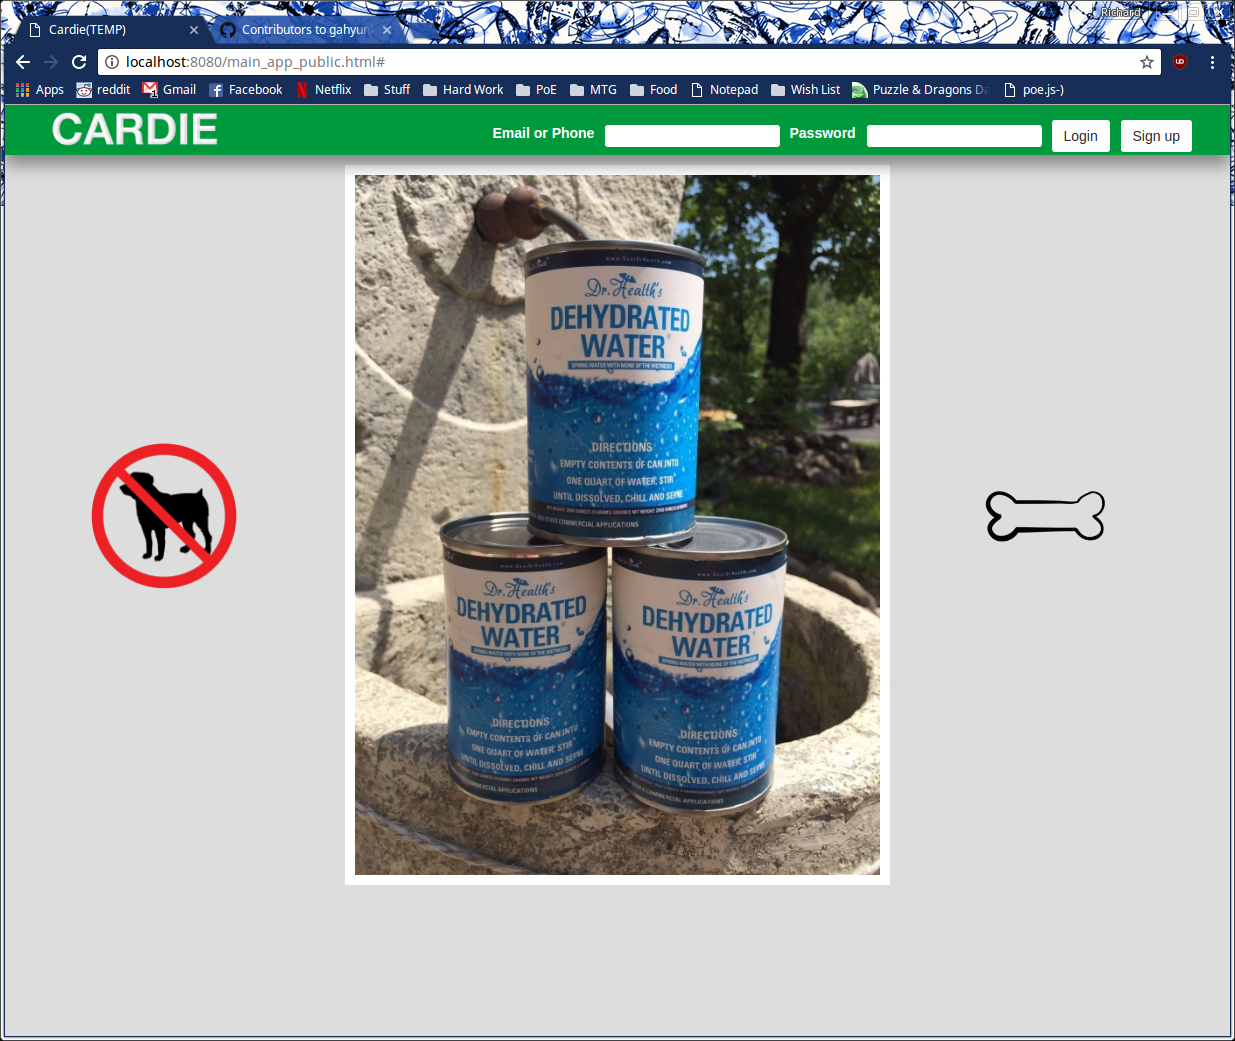
\includegraphics[scale=.4]{screen_00}}

\pagebreak

\noindent Once logged in, then the navbar switches to the private version and the user can access other features of the web application: \\

\centerline{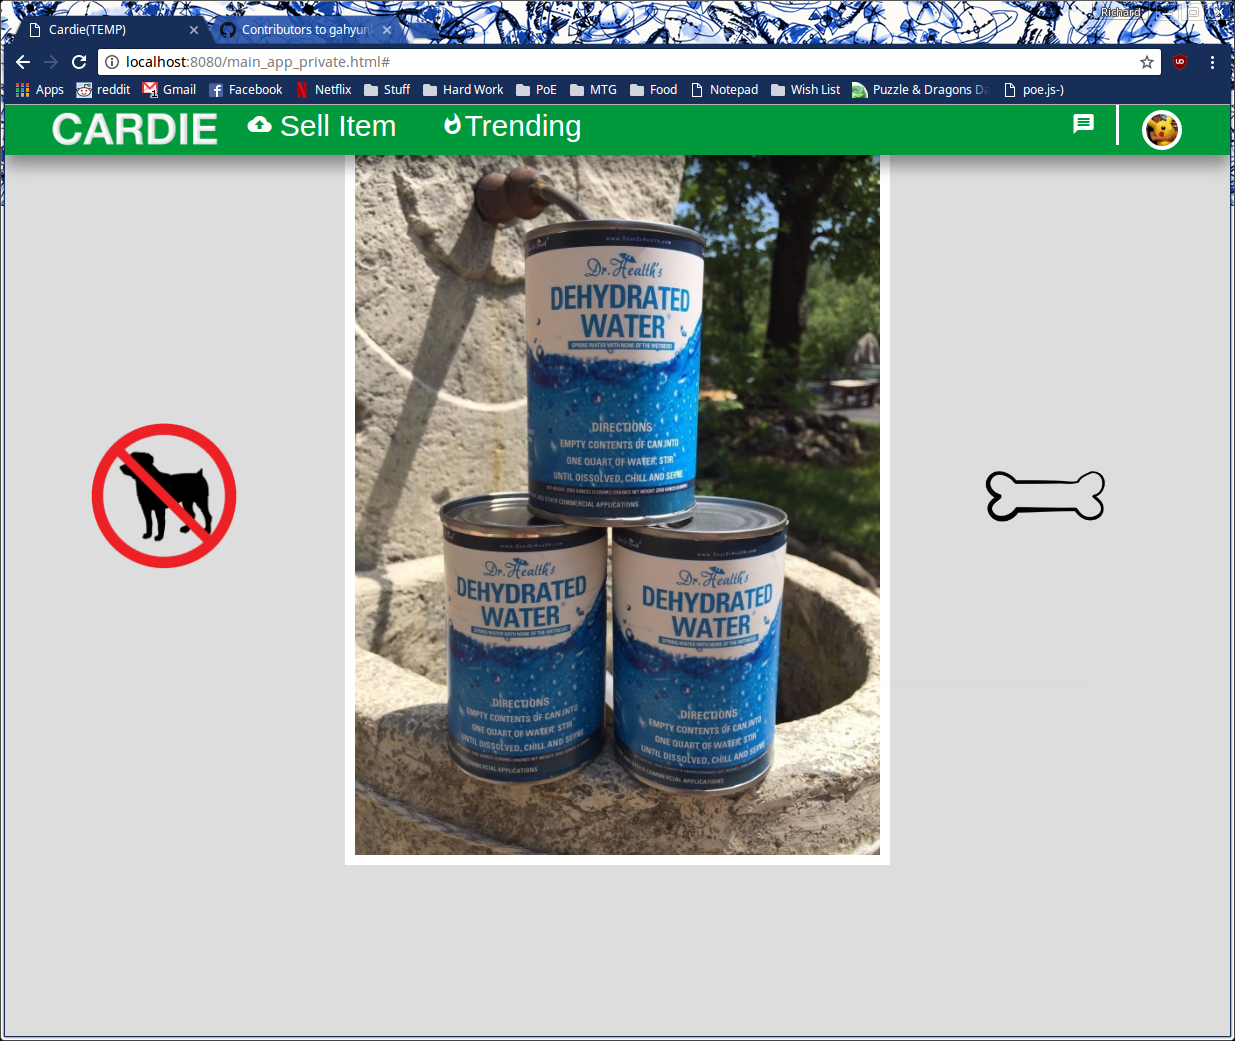
\includegraphics[scale=.4]{screen_01}}

\pagebreak

\noindent If the user clicks on the item image, they open a popup with more information on the item. Currently it is in a new page, but we intend to display it as a javascript popup: \\

\centerline{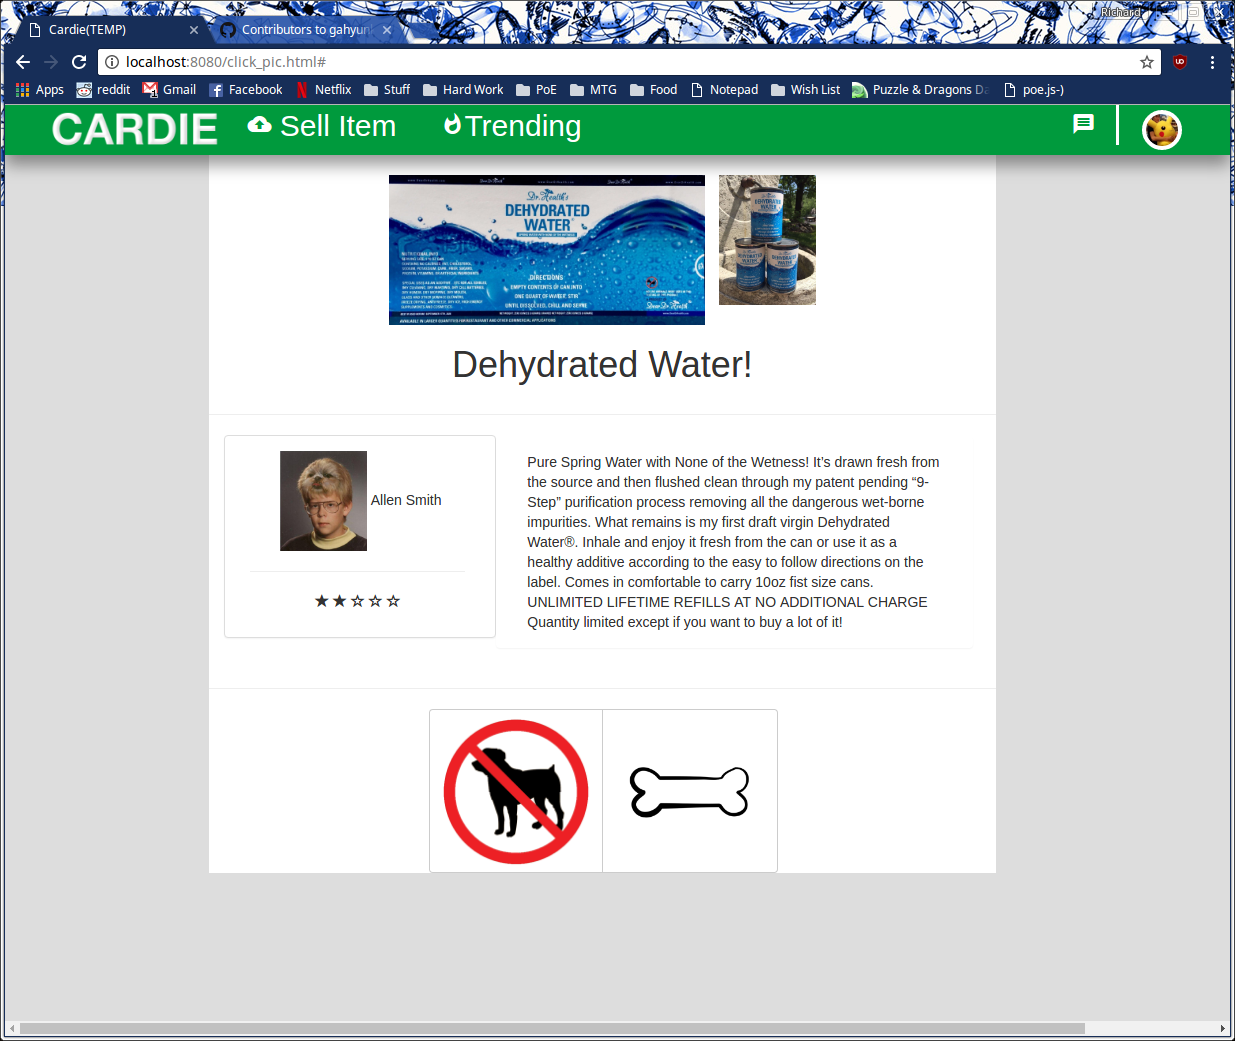
\includegraphics[scale=.4]{screen_03}}

\pagebreak

\noindent Clicking on the "Sell Item" button on the navbar brings the user to a form where they can submit an item to sell: \\

\centerline{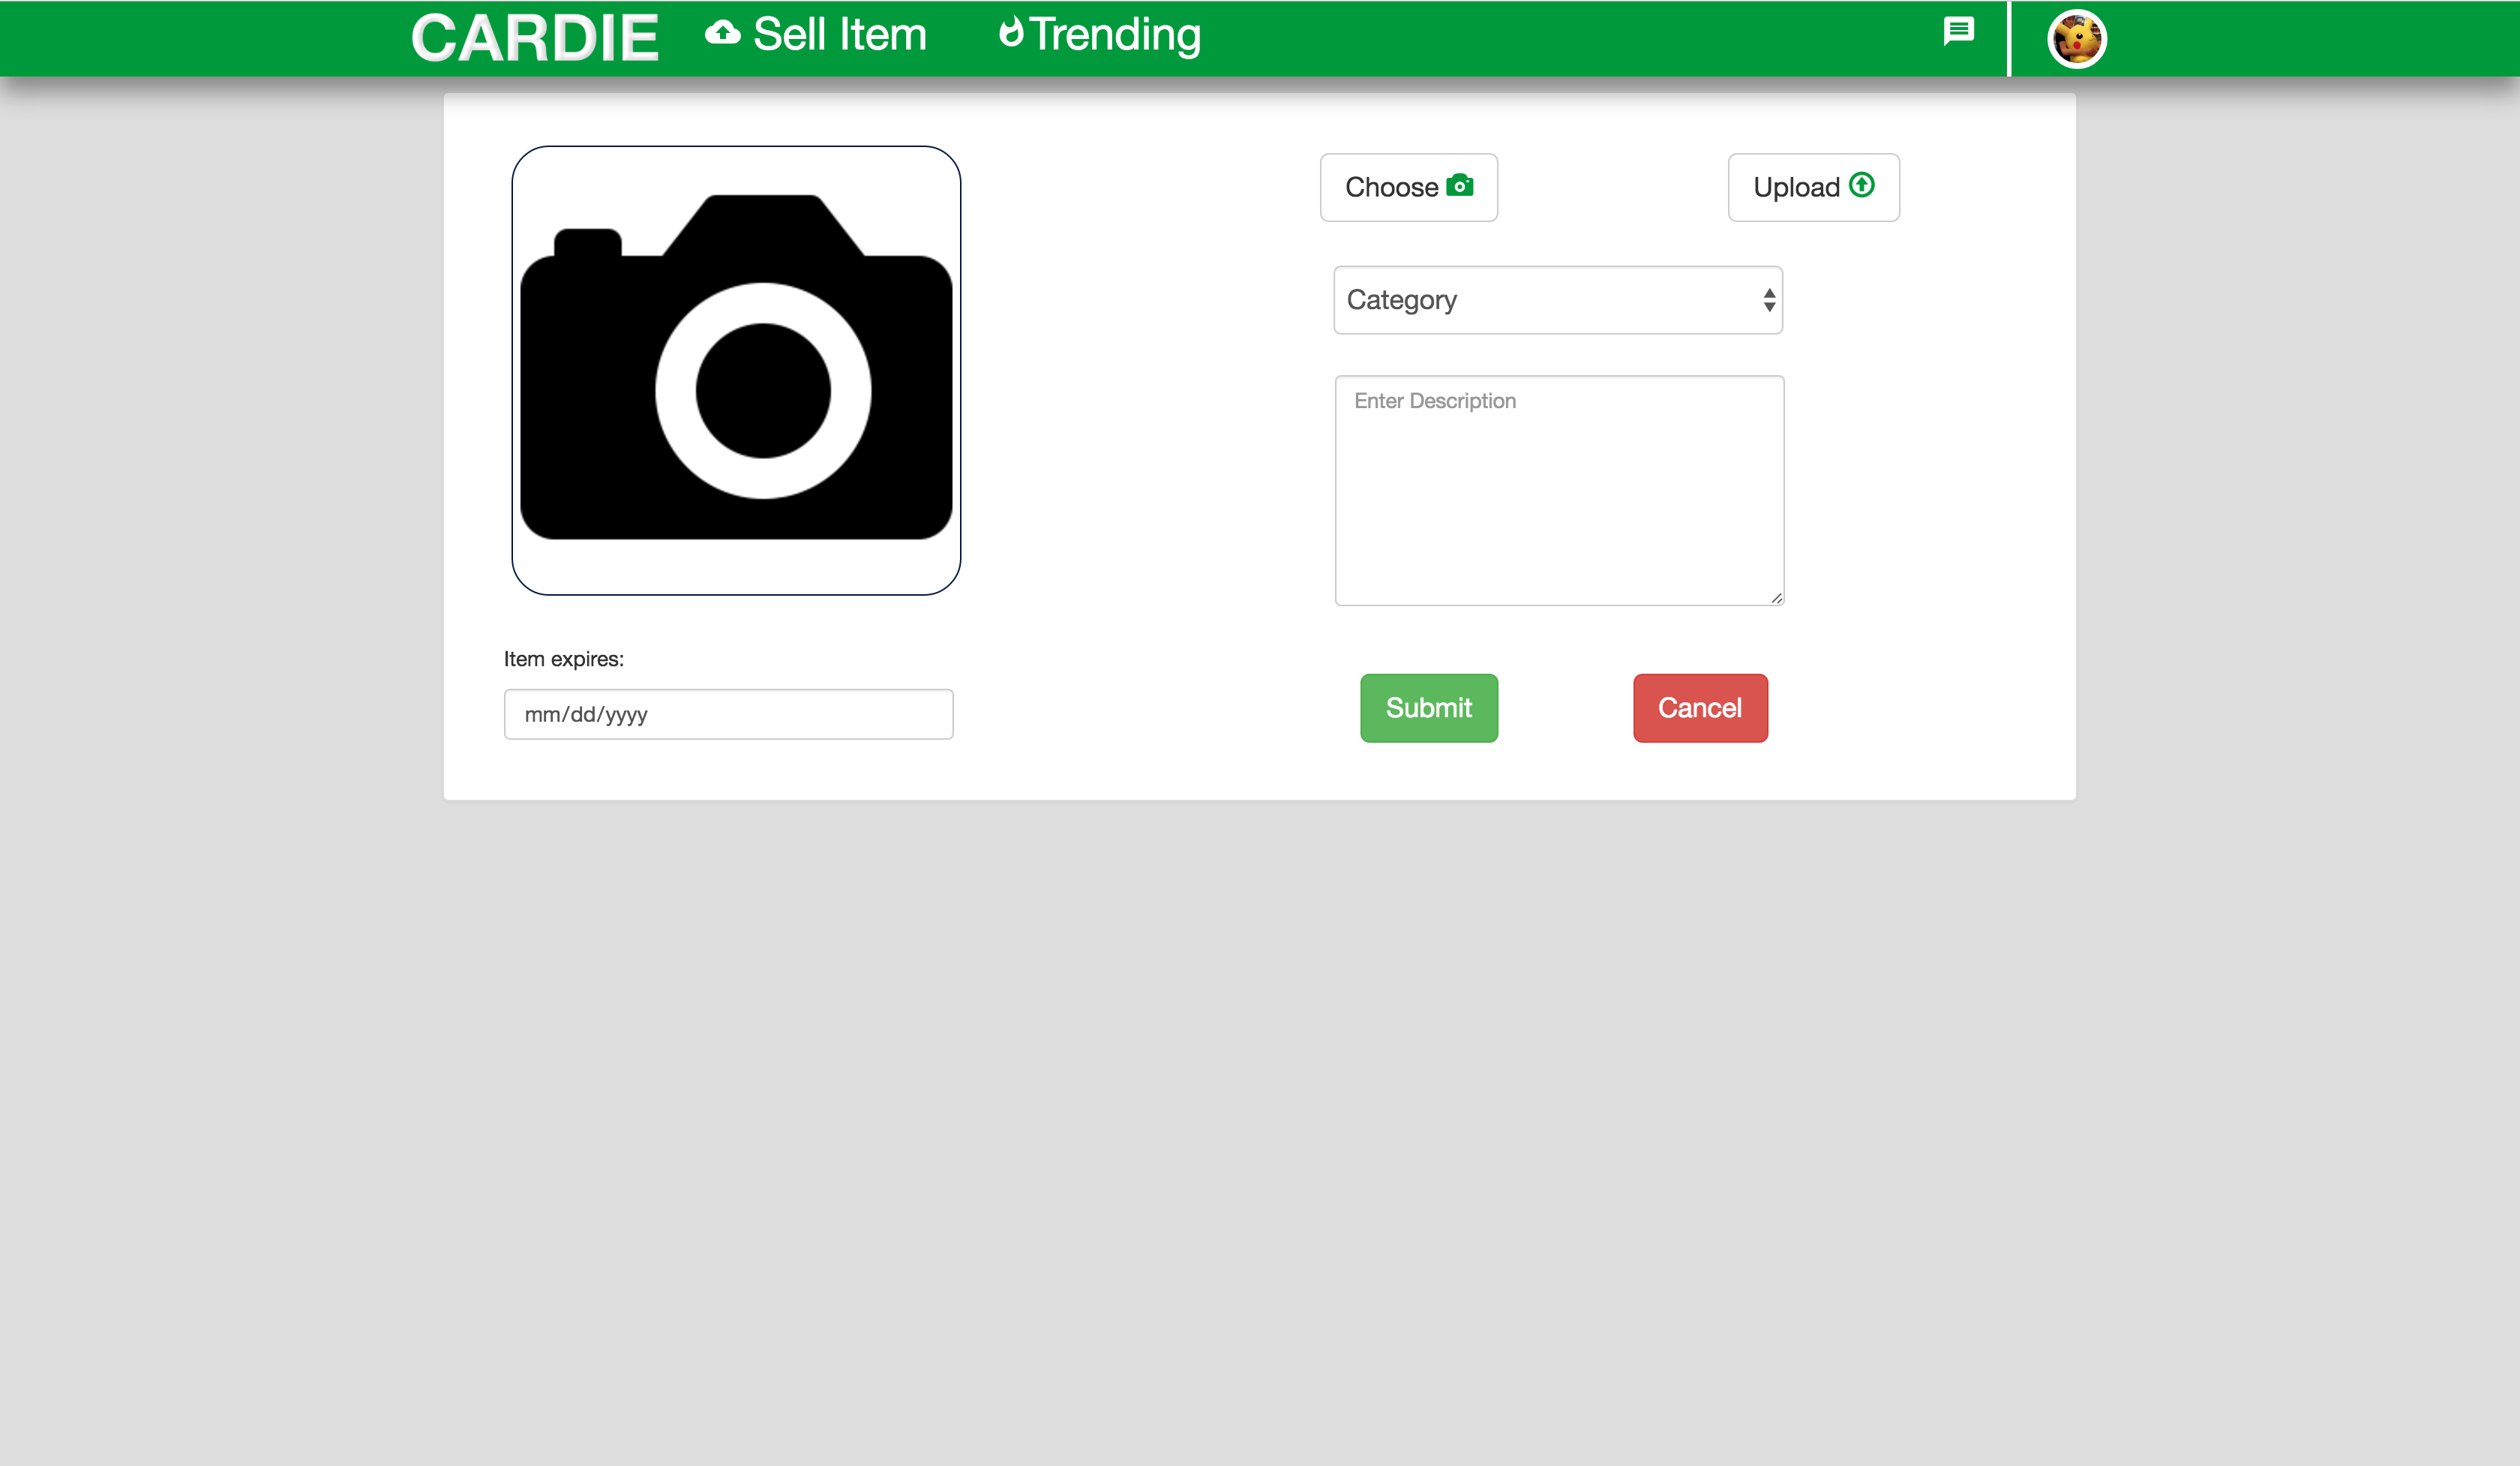
\includegraphics[scale=.4]{screen_07}}


\pagebreak

\noindent Clicking on the "Trending" button on the navbar brings the user to a page where they can browse through items that are currently trending, sorted by category. Clicking on a category allows the user to see more: \\

\centerline{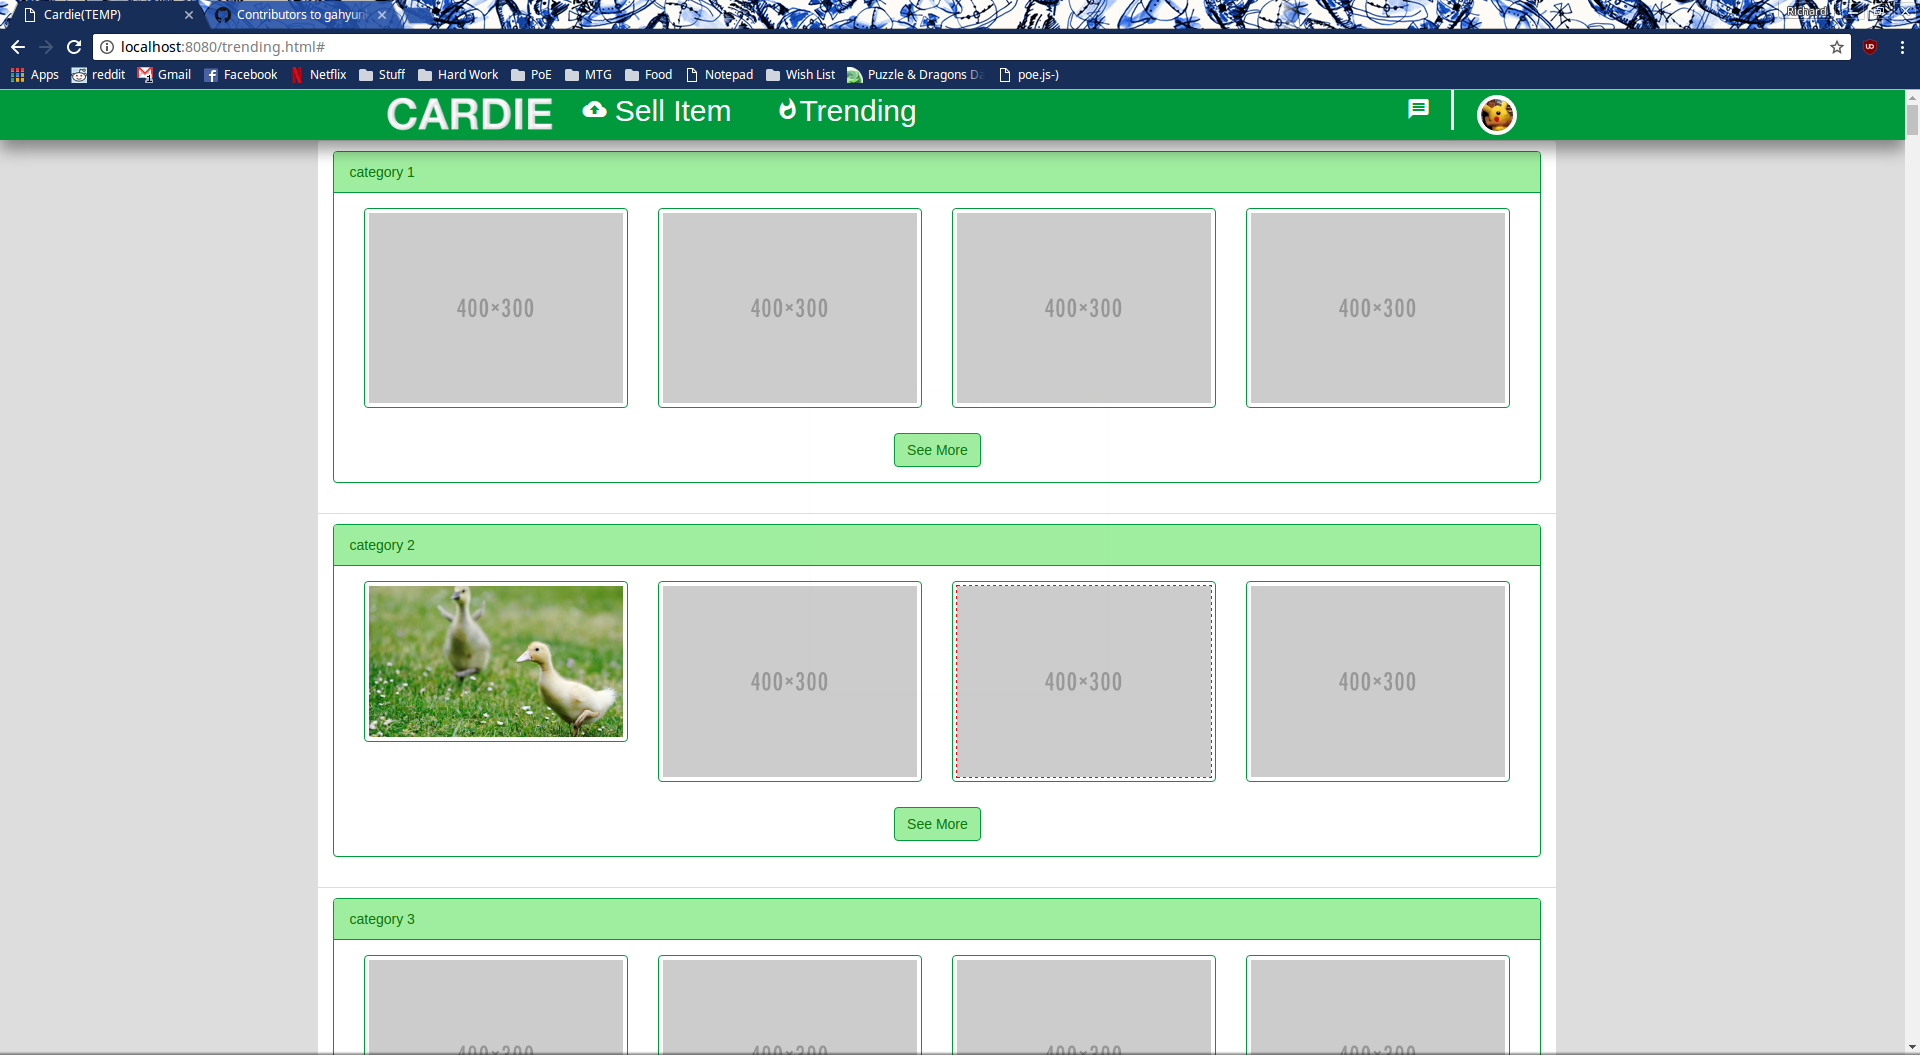
\includegraphics[scale=.25]{screen_05}}

\pagebreak

\noindent On the right side of the navbar, the message button brings the user to a chat interface where the user can interact with potential buyers and sellers: \\

\centerline{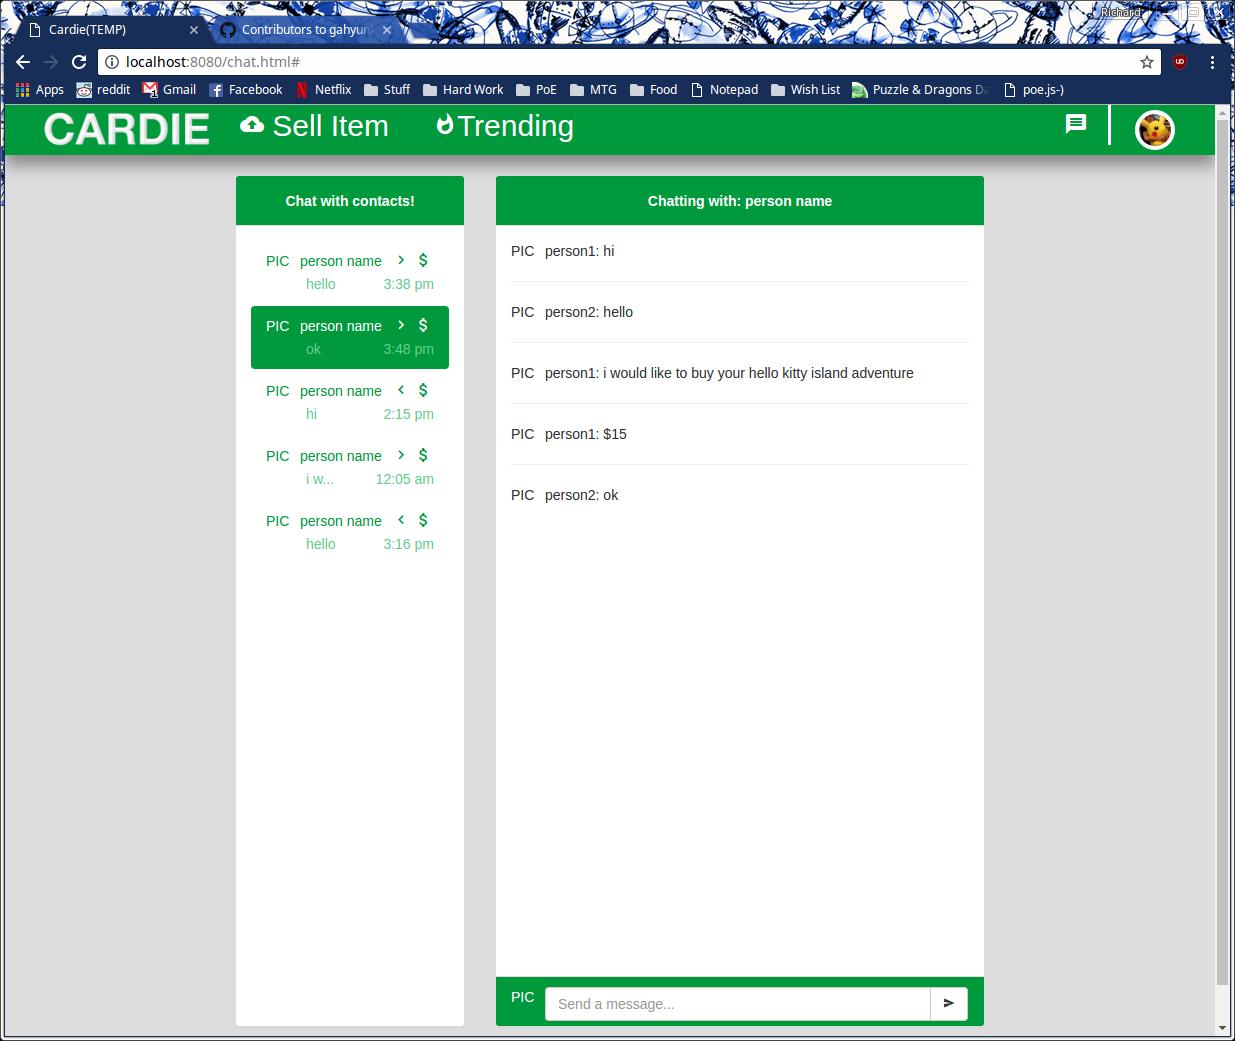
\includegraphics[scale=.4]{screen_04}}

\pagebreak

\noindent Hovering over the profile picture on the far right side of the navbar displays a drop down menu which contains some administrative links, one of which is the user profile settings: \\

\centerline{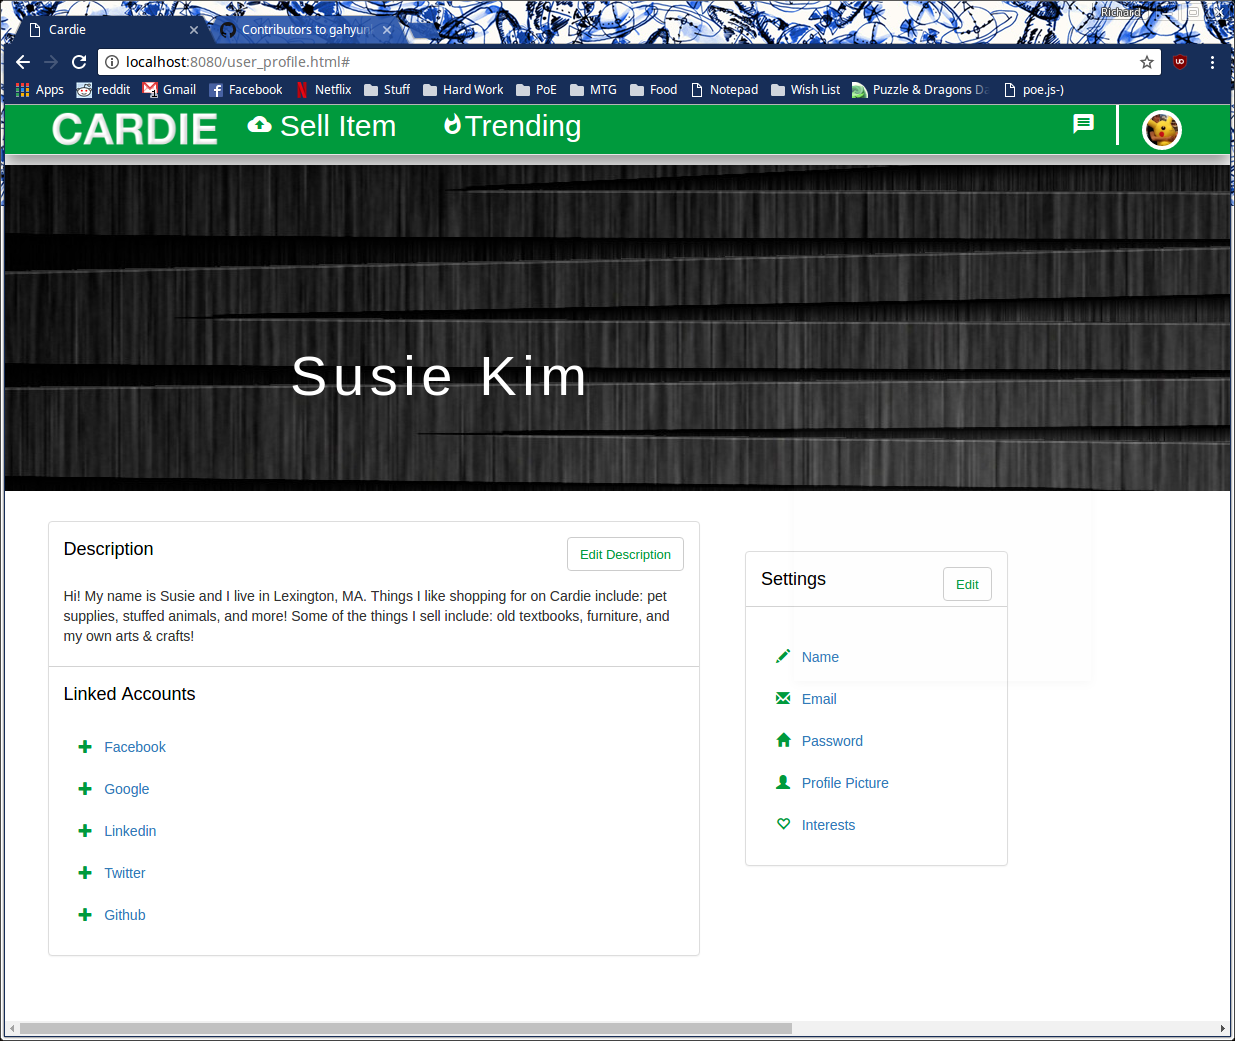
\includegraphics[scale=.4]{screen_06}}

\pagebreak

\noindent Another administrative link that the user has access to is the item management page, which allows the user to administrate the items that they have for sale: \\

\centerline{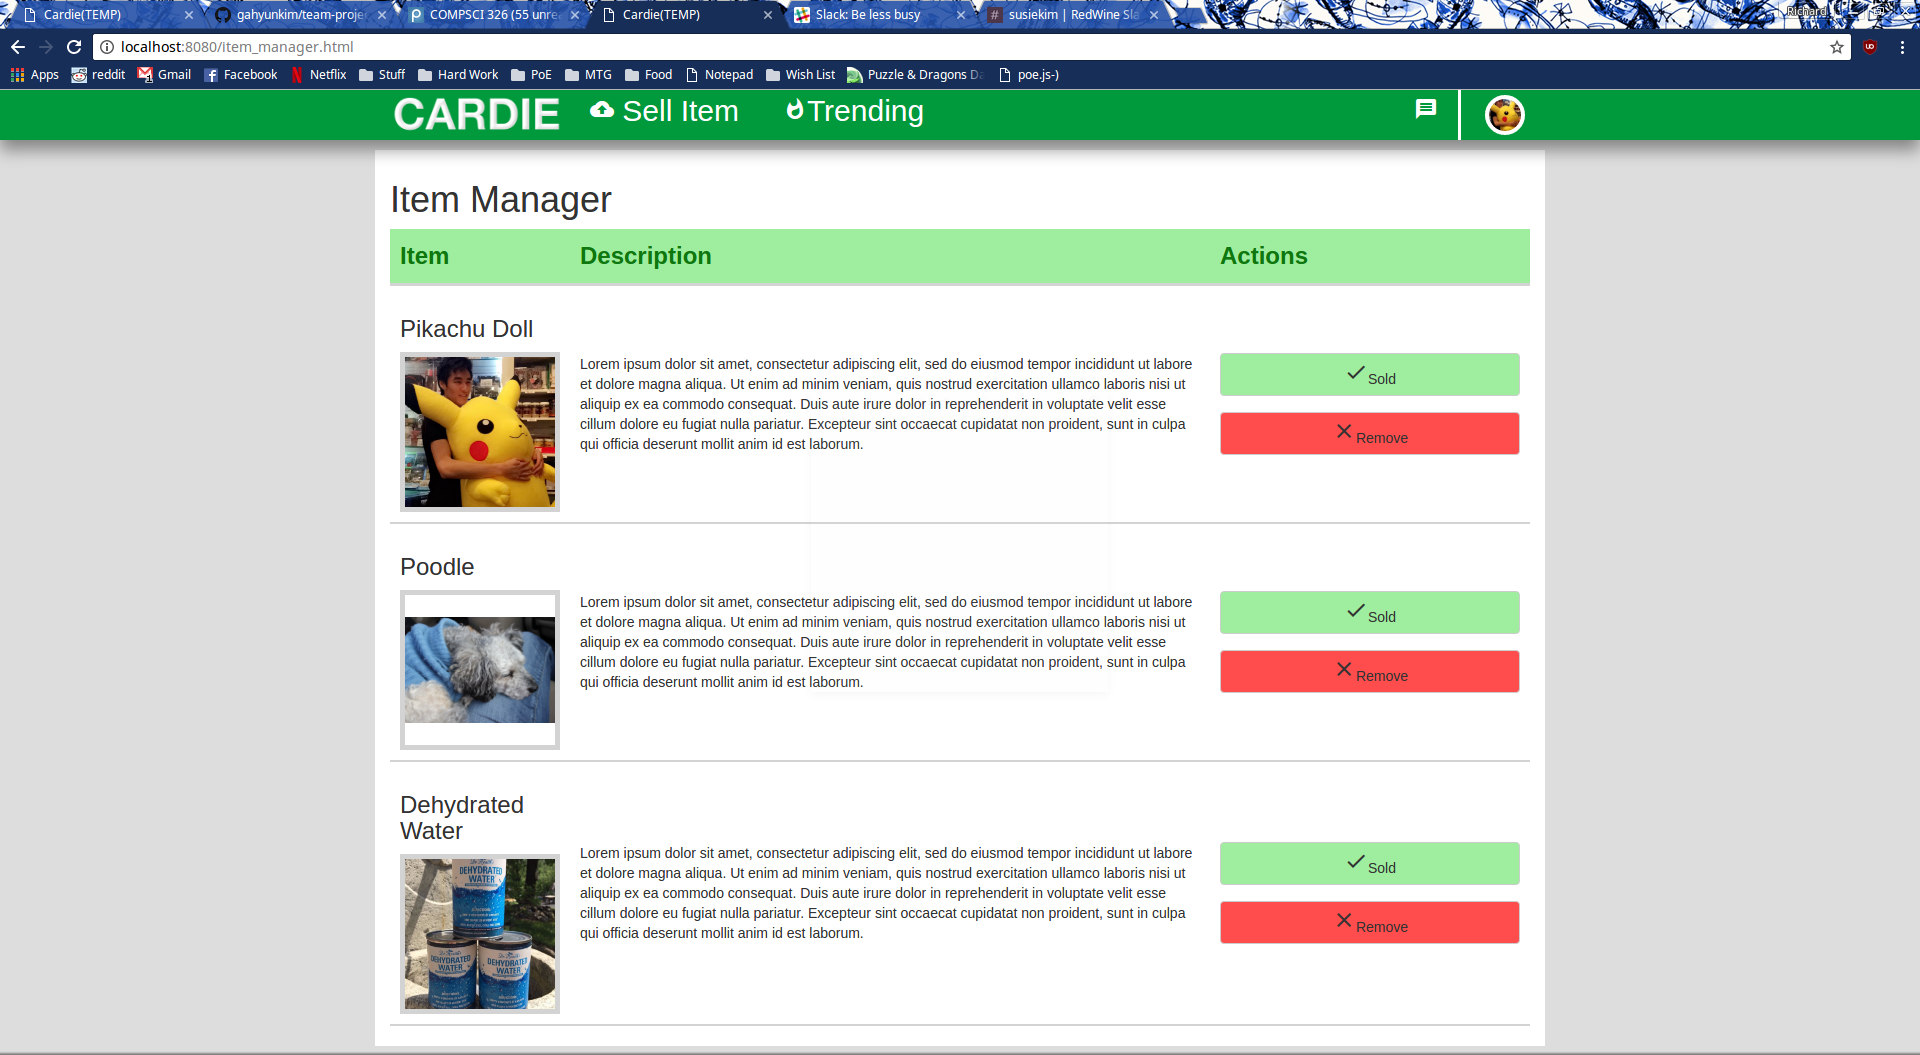
\includegraphics[scale=.25]{screen_09}}

\pagebreak

\noindent RESPONSIBILITIES\\
Francis Phan\\
\indent - Navigation bar (public and private)\\
\indent - Item Manager UI\\
\indent - main.css\\
Richard Cui\\
\indent - Chat UI\\
\indent - Written Report\\
Gahyun (Susie) Kim\\
\indent - User Profile \\
Greg McGrath\\
\indent - Main UI (public and private)\\
Roman Ganchin\\
\indent - Trending Items UI\\
Daanial Ahmed\\
\indent - Upload Item UI\\




\end{document}